% pre-amble section
\documentclass[final, letterpaper, 10 pt, conference, twocolumn]{IEEEtran}

\usepackage[utf8]{inputenc}
\usepackage{geometry}
\usepackage{hyperref}
\usepackage{graphicx}
\graphicspath{ {Images/} }
\usepackage{listings}
\usepackage{xcolor}
\usepackage{fancyvrb}
\usepackage[backend=bibtex]{biblatex}

\bibliography{references.bib}

\lstdefinestyle{DOS}
{
    backgroundcolor=\color{black},
    basicstyle=\scriptsize\color{white}\ttfamily
}

\title{Herbert\\Autonomous Robotic Rubik's Cube Solver}
\author{
    Jonathan Whitaker, Dylan Lytle, Matt Frandsen, Li Lao\\
    \textit{Dept. of Electrical and Computer Engineering, University of Utah}\\
}

\date{December 2015}
% end of pre-amble

% document content
\begin{document}

\maketitle

\begin{abstract}
Project Herbert is an autonomous robotic Rubik's Cube solver that is composed of a complex network of mechanical and electrical devices. In this project our team interfaced with these complex mechanical and electrical devices so as to design and create an autonomous robot that is capable of solving a Rubik's cube within two minutes of time.  This project is an integration of various technologies including: mechanical actuators, electrical stepper motors, single-board computers, field-programmable gate arrays, and video cameras.
\end{abstract}

\section{Introduction}
\label{sec:intro}
The goal of this project was to create an autonomous robotic Rubik's Cube solver through the integration of several components. The main components integrated into our project include video cameras, electrical stepper motors, mechanical actuators, a single-board computer (SBC), and field-programmable gate arrays (FPGAs). A video camera connects to the computer through standard universal serial bus (USB) 2.0 protocol \cite{USB2.0}. The video camera is responsible for capturing the initial configuration of the Rubik's Cube, and the single board computer is responsible for processing the video frame information and generating a matrix model for the initial state of the cube. After generating a matrix model for the initial cube, the computer applies Kociemba's algorithm \cite{Kociemba} (an optimal algorithm used to solve a Rubik's Cube) to generate a solution sequence that can be processed sequentially. The solution sequence that Kociemba's algorithm returns is in the standard notation used in Rubik's Cube discussion and theory (see Appendix \ref{sec:Appendix A}). As each solution sequence is processed, the computer communicates through an RS232 serial connection to an FPGA control board which drives the mechanical actuations and stepper motor rotations needed to physically manipulate the cube. The FPGA acts as a system control board and is responsible for controlling the actions of two motor control boards and a relay board used to trigger the mechanical actuators.

\begin{figure}[!ht]
\centering
\includegraphics[scale=0.25]{"Rubik's Cube Positioning".png}
\caption{Initial ideal cube image capture}
\label{fig:Camera Positioning}
\end{figure}

\begin{figure}[!ht]
\centering
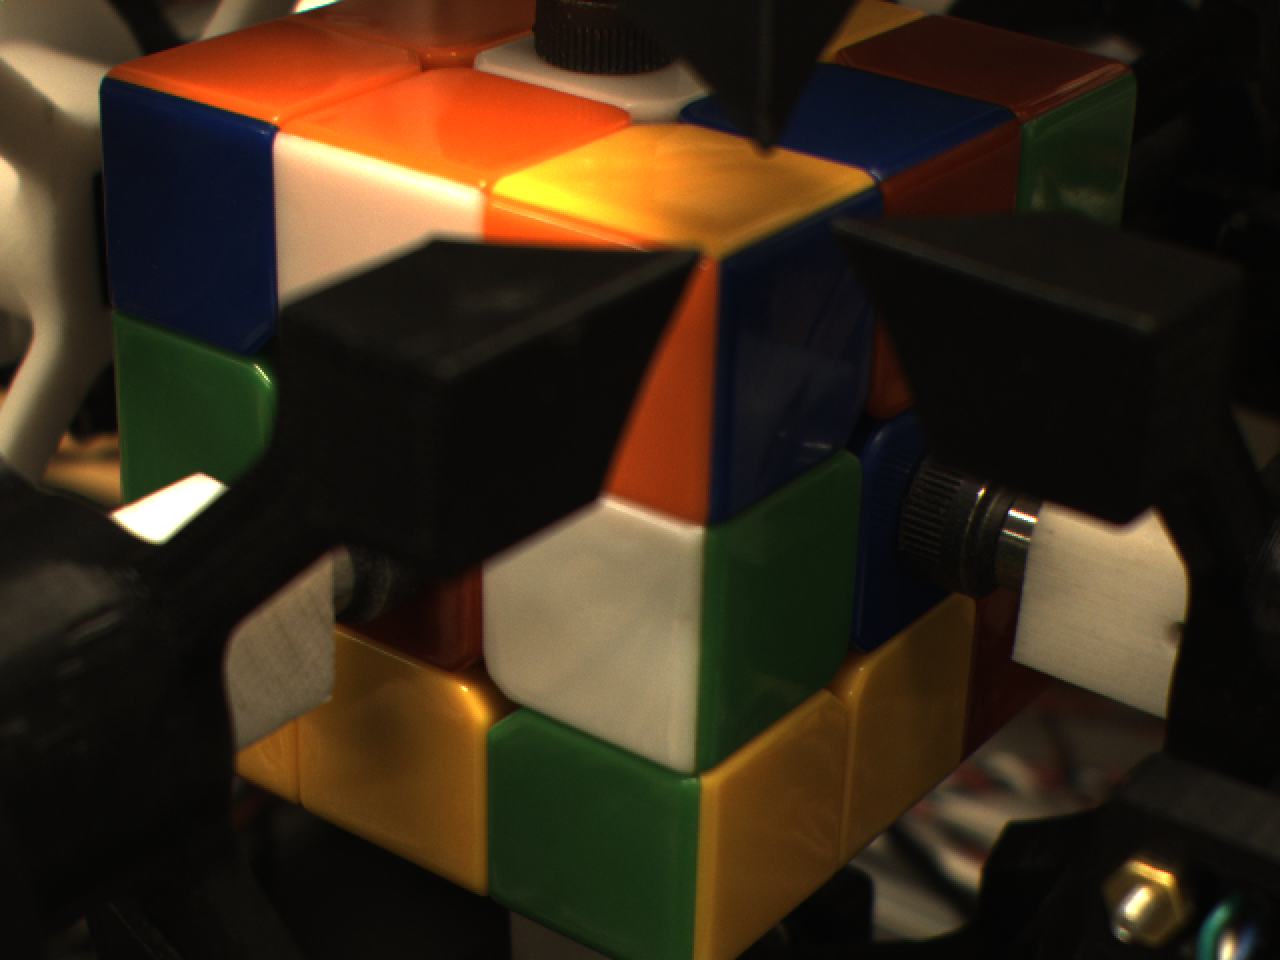
\includegraphics[scale=0.15]{actual_cube_capture.png}
\caption{Obscured cube image capture}
\label{fig:Obscured Cube}
\end{figure}

\section{Software Implementation}
\label{sec:Software Implementation}

The project uses a good software implementation. (This won't be included in the actual report)

\subsection{Image Processing}
The image processing functionalities aims to capture the state of the cube using camera. The criteria for evaluating the success of the image processing implementation is robustness and speed of the algorithm.

\subsubsection{Point Grey Camera and FlyCapture Software Development Kit}
The cameras was supplied by Point Grey and interfaced through FlyCapture software development kit (SDK). The FlyCapture SDK was implemented in C. Cython, an optimised static compiler for Python to C, was used to bind with the SDK from Python.  The FlyCapture SDK  provided high configurability and flexible interface for the cameras which was adjust for image capturing mode and synchronizing image buffer retrieval. 

The initial design was to use two camera connected to a SBC through a standard USB 2.0 connection. Each one of these cameras is responsible for capturing exactly three of the six faces of the cube with a view as shown in Fig. \ref{fig:Camera Positioning}. However, various parts from the mechanical system obscured the view a majority of the facelets on the three faces. Additionally, the challenges dealing with color recognition made using the initial camera configuration even more complex.

The final camera configuration used a single camera to capture the entire state of a Rubik's Cube as shown in Fig. \ref{fig:Obscured Cube}. A static sequence of rotation using the mechnical system is used to capture the cube in various configurations until all the facelets on the cube has been visible one or more times. The cube is then returned to its original state and the collection of images are saved off for later processing.

\subsubsection{Cube Orientation}
\subsubsection{Color Recognition}
After all 
\paragraph{Color Space}
Several factors affects the robustness of the color recognition. 
\paragraph{Categorization Algorithm}


\subsection{Kcube and Solution Sequence}
\begin{figure*}[!ht]
\begin{center}
\begin{BVerbatim}
             |************|
             |*U1**U2**U3*|
             |************|
             |*U4**U5**U6*|
             |************|
             |*U7**U8**U9*|
             |************|
|************|************|************|************|
|*L1**L2**L3*|*F1**F2**F3*|*R1**R2**F3*|*B1**B2**B3*|
|************|************|************|************|
|*L4**L5**L6*|*F4**F5**F6*|*R4**R5**R6*|*B4**B5**B6*|
|************|************|************|************|
|*L7**L8**L9*|*F7**F8**F9*|*R7**R8**R9*|*B7**B8**B9*|
|************|************|************|************|
             |************|
             |*D1**D2**D3*|
             |************|
             |*D4**D5**D6*|
             |************|
             |*D7**D8**D9*|
             |************|
\end{BVerbatim}
\end{center}
\caption{Rubik's Cube matrix representation}
\label{fig:matrix layout}
\end{figure*}

\begin{table}[!ht]
\caption{Cubelet color to ASCII character mapping}
\label{table:cubelet representation}
\centering
\begin{tabular}{|c|c|}
\hline
\textbf{COLOR} & \textbf{CHARACTER} \\ \hline
WHITE          & `W'              \\ \hline
RED            & `R'              \\ \hline
BLUE           & `B'              \\ \hline
GREEN          & `G'              \\ \hline
ORANGE         & `O'              \\ \hline
YELLOW         & `Y'              \\ \hline
\end{tabular}
\end{table}

\subsection{Kcube and the Solution Sequence}
\label{sec:Kcube}
Kcube is a C++ application developed by Greg Schmidt that utilizes Kociemba's two-phase algorithm which uses two stages of an iterative depth first search algorithm \cite{TheTwo-PhaseAlgorithm}. We utilized the Kcube application to generate the solution sequence needed to solve the Rubik's Cube that was captured during the image processing phase. The matrix model generated from the image processing phase allows us to provide Kcube's command-line interface with the cube representation needed to generate a solution sequence. Kcube's command-line interface takes six parameters, one for each face of the cube. The values for these parameters are the color characters at each of the cubelet locations for that face (as seen in Fig. \ref{fig:matrix layout}). For example, to solve the scrambled cube shown in Fig. \ref{fig:scrambled cube} you invoke Kcube with the following command:

\begin{lstlisting}[style=DOS]
c:>kcube L:GGWWOWBRB
         F:GWGBGYWBO
         U:YOOOWYROY
         D:ORGWYYYRB
         R:OGBBRYWRR
         B:YBROBGWGR
\end{lstlisting}

Kcube processes the input parameters and generates a sequence of twenty-three or less moves (see Appendix \ref{sec:fundamental moves}) that, when applied to the cube, will solve the cube. Each move is mapped to a unique character or set of characters (see Table \ref{table:moves table}), and these characters are transmitted over an RS232 serial connection to the FPGA control board, at which point the control board takes responsibility for controlling the electro-mechanical stepper motors and mechanical actuators needed to physically manipulate the cube.


\begin{figure}[!hb]
\centering
\includegraphics[scale=1.0]{"Scrambled Cube".jpg}
\caption{A scrambled cube}
\label{fig:scrambled cube}
\end{figure}

\begin{table}[!ht]
\caption{Cube moves to character set mapping}
\label{table:moves table}
\centering
\begin{tabular}{|c|c|c|c|c|c|}
\hline
\textbf{MOVE} & \textbf{CHAR} & \textbf{MOVE} & \textbf{CHAR} & \textbf{MOVE} & \textbf{CHAR} \\ \hline
F             & F              & R             & R              & D             & D             \\ \hline
F'            & Fb              & R'            & Rb              & D'            & Db            \\ \hline
F2            & F2              & R2            & R2              & D2            & D2             \\ \hline
L             & L              & U             & U             & B             & B             \\ \hline
L'            & Lb              & U'            & Ub             & B'            & Bb             \\ \hline
L2            & L2              & U2            & U2             & B2            & B2             \\ \hline
\end{tabular}
\end{table}


\subsection{Serial Communication and Command Format}

\section{Hardware Implementation}
\subsection{Mechanical Actuators}
\label{sec:Mechanical Actuators}
Herbert employs a six arm design to physically manipulate the cube. One arm for each face of the cube. In order to achieve a six arm design, each arm actuates in and out so as to avoid conflict
with the other arms. This actuation process is a time critical component of
the design.  We initially planned on implementing the
arm actuation with motors.  However, preliminary testing showed that using
motors to convert rotary motion into linear motion is too slow, and using a linear motor
actuator is too costly. We decided that pneumatic actuation is the solution to this problem.  Each of the arms is attached to a double action pneumatic air cylinder as show in Fig. \ref{fig:Pneumatic Air Cylinder}.

\begin{figure}[!ht]
\centering
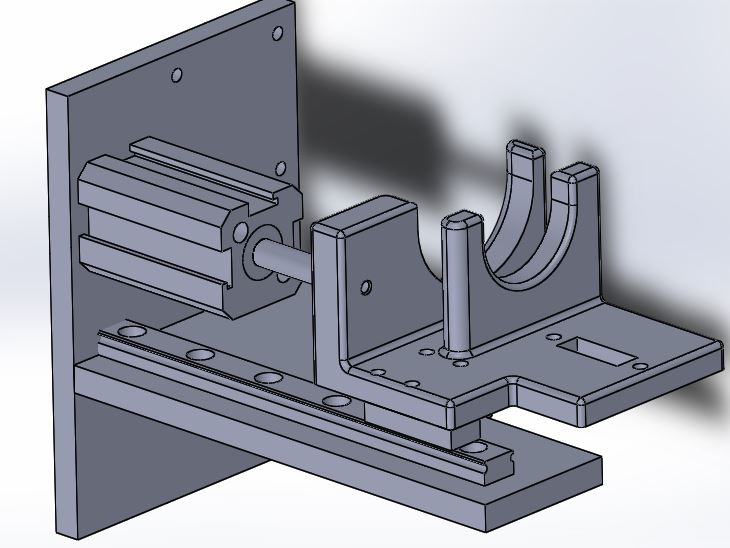
\includegraphics[scale=0.28]{AirCylinder.jpg}
\caption{Pneumatic Air Cylinder}
\label{fig:Pneumatic Air Cylinder}
\end{figure}

The FPGA control board is responsible for controlling a relay control board (see Fig. \ref{fig:System Block Diagram}) which controls coaxial pairs of air cylinders. The actuation distance for each control arm is fixed. The coaxial pairs of arms are kept in an extended or retracted position, depending on the current move being executed. Potential optimizations and more stable cube manipulations  are obtained by simultaneously extending and retracting coaxial pairs of arms. The linear actuation motion allows two coaxial pairs of
arms to extend, thus encasing two sides of the cube in the sockets of the arms. After a pair of arms extend,
a stepper motor spins the arm corresponding to the appropriate move from the solution sequence (see section \ref{sec:Stepper Motors}). Each air cylinder is provided approximately 40-60 psi supplied from an air compressor. To protect against any arm collisions, only one pair of arms is in the extended position at any given time.

Initially our design incorporated mechanical switches that would be triggered by physical contact of the arm assembly.  These switches were mounted on the assembly in such a way that contact would occur in either the extended or retracted arm positions.  The goal of the switch based design was to remove an element of manual timing approximation.  By using the switches we would know the position of each arm at all times.  Taking advantage of this, there would be a much smaller hard coded delay, or potentially no delay.  However, due to time constraints as well as accuracy issues because of inconsistent and difficult mounting, we chose not to implement the switches in the final design.   
 
If we were to continue the project there are many improvements and optimizations that could be made. The first optimization would be to implement the switch design we initially planned on.  Improving the robustness of the switches would help reduce the time the mechanical motion takes. This would reduce the overall time to completion, because the mechanical motion is the most time intensive component of the solution. 
Another mechanical optimization that would help reduce the time to completion is to modify the arm.  The image processing was a very difficult component of this project, because the arm assembly was obtrusive to the view of the cube for the cameras.  Our thought is to remove two of the four prongs of each arm.  This modification would give the cameras a more clear view of the cube, as well as potentially giving us the ability to actuate in and out more quickly, because potential arm collisions would be reduced.

\begin{figure}[!ht]
\centering
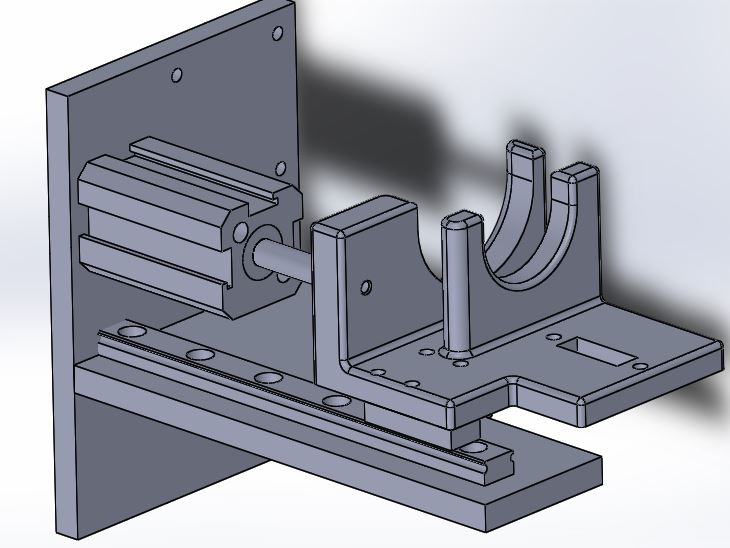
\includegraphics[scale=0.28]{AirCylinder.jpg}
\caption{Pneumatic Air Cylinder and 3D Printed Axel Support}
\label{fig:Pneumatic Air Cylinder}
\end{figure}

\subsubsection{Electro-mechanical Stepper Motors}
\label{sec:Stepper Motors}
Each actuating arm has a stepper motor which is responsible for rotating a single face. A stepper motor rotates a face either 90 degrees or 180 degrees clockwise or counter-clockwise based on the solution move that is being processed (as specified in Appendix \ref{sec:Appendix A}). A 3D printed axle (as seen Fig. \ref{fig:Stepper Motor Arm}) is fastened to the stepper motors. This axle twists a 3D printed arm piece in order to spin a face of the Rubik's Cube.

\begin{figure}[!ht]
\centering
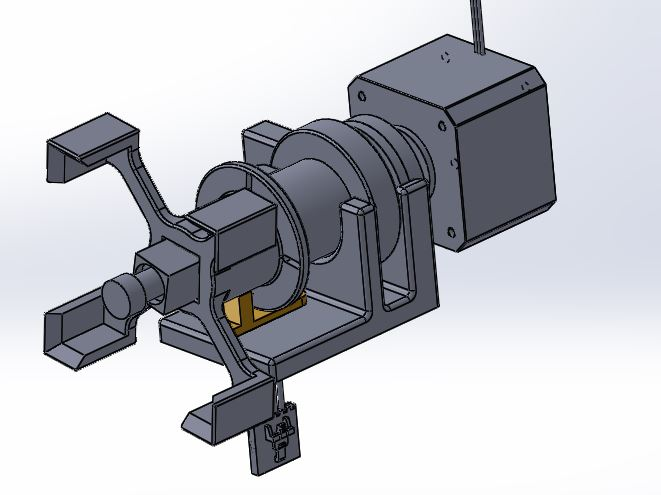
\includegraphics[scale=0.30]{StepperMotorArm.jpg}
\caption{Stepper Motor Arm Assembly}
\label{fig:Stepper Motor Arm}
\end{figure}

Each stepper motor is driven by a motor control board which is controlled by the FPGA control board (see Fig. \ref{fig:System Block Diagram}). The motor control boards contain a motor driver chip for each stepper motor. The FPGA control board is responsible for controlling the angular and temporal timing of each stepper motor rotation.

\subsection{Infrared Break Sensors}
\label{sec:Infrared Break Sensors}
Rotations must end at a 90 degree angle so as to not interrupt the rotation of another arm.  These exact angles are hard to accomplish by counting steps, because it is difficult to detect whether steps are skipped.  To compensate for this we used infrared break sensors like that shown in Fig. \ref{fig:Infrared Break Sensor}. Each arm assembly has an infrared sensor (see Fig. \ref{fig:Stepper Motor Arm}). The infrared sensor is broken at all angles that are not a multiple of 90 degrees. These break sensors are monitored and controlled through the motor control boards.

\begin{figure}[!ht]
\centering
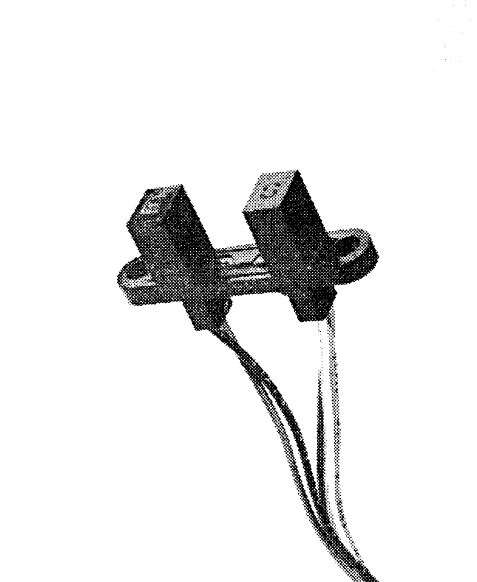
\includegraphics[scale=0.28]{InfraredBreakSensor.jpg}
\caption{Infrared Break Sensor}
\label{fig:Infrared Break Sensor}
\end{figure}

\subsection{Arm Progression}
\label{sec:Arm Progression}
The 3D printed arm piece at the end of each arm assembly (see Fig. \ref{fig:Stepper Motor Arm}) underwent a great progression. Fig. \ref{fig:Arm Progression} highlights the progression of the arm pieces from left to right. The first iteration was a simple arm that had a square socket and connected directly to the stepper motor without any intermediate axel piece.  The inner part of the socket had chamfered edges to correct for any error in alignment.  The second iteration included tabs for break sensor detection, and it was elongated to accommodate the length of the center pin.  We also modified the socket into four prongs. This allowed better visibility of the cube for the image processing. In the last arm revision we changed from tabbed break sensor detection to slits. This improvement allowed more precise angle detection.  We also shortened the arm, added more chamfered edges for minor alignment error corrections, and included slight height changes to fit the slider piece and circular cutouts to avoid arm collisions.

\begin{figure}[!ht]
\centering
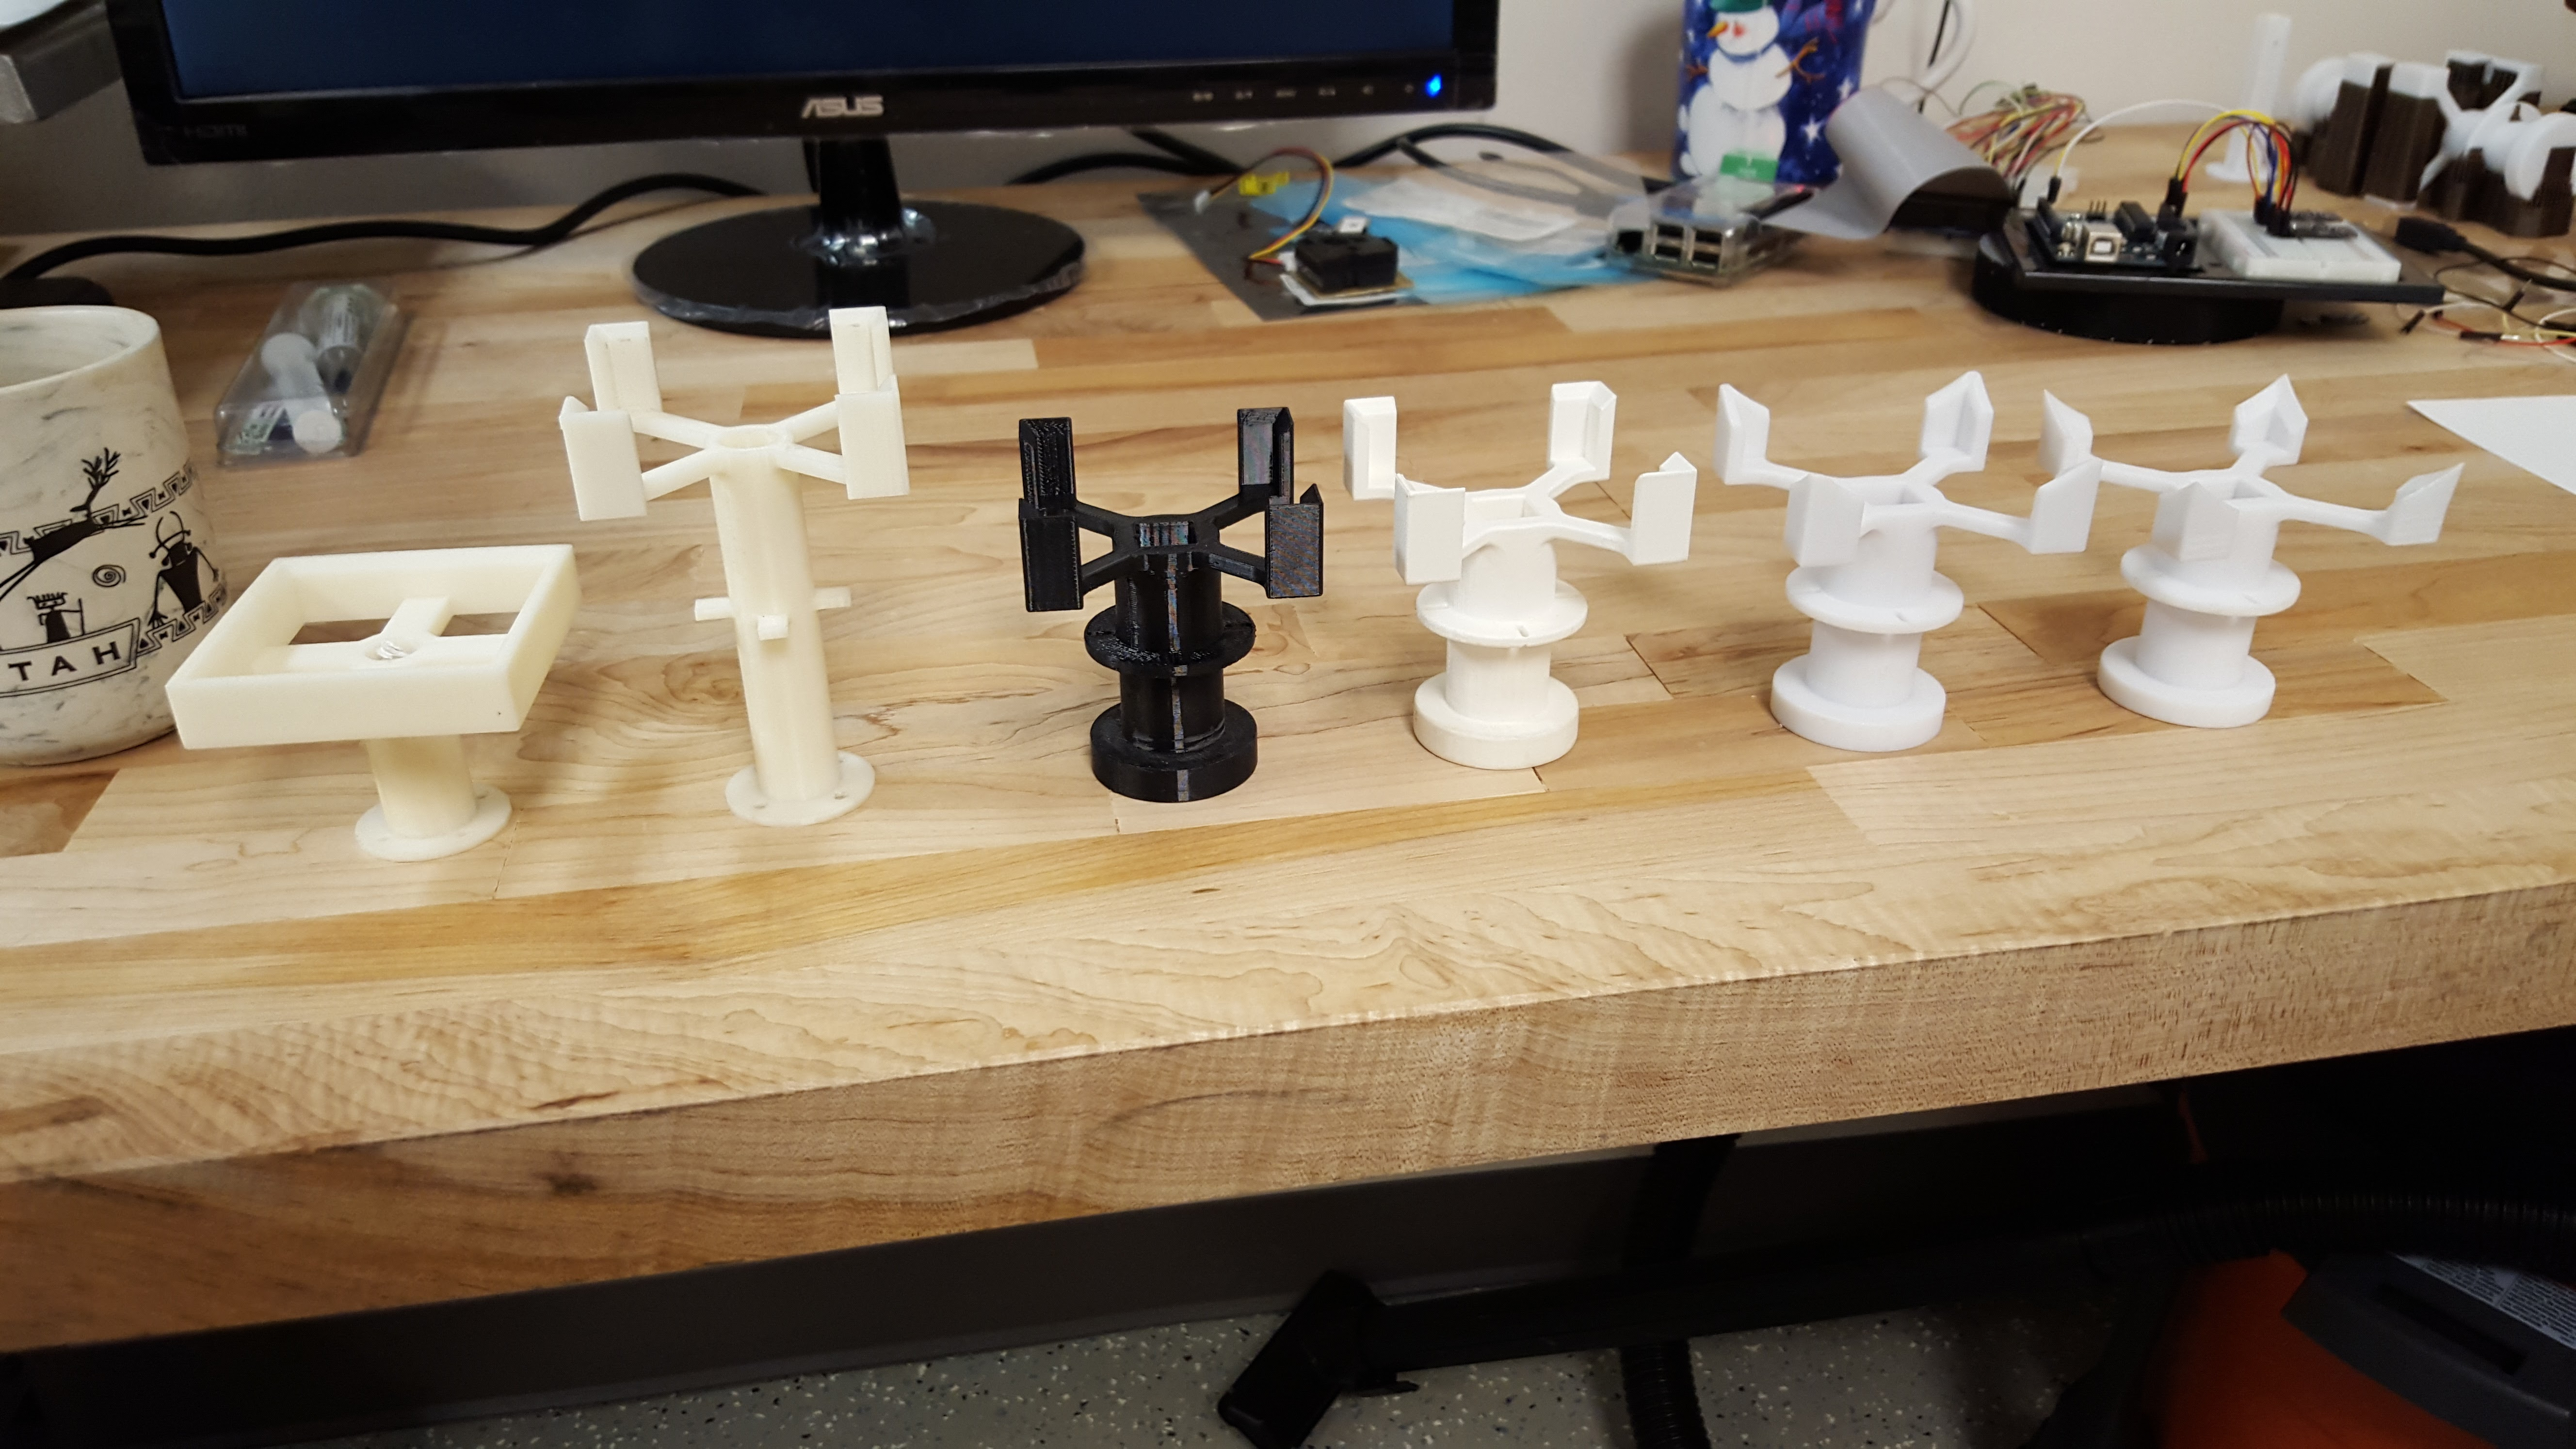
\includegraphics[width=\linewidth]{ArmProgression.jpg}
\caption{Arm Progresssion}
\label{fig:Arm Progression}
\end{figure}


\section{Firmware}
Table \ref{table:CMDS} is a detailed list of the commands we used for this project.

Default behavior of the stepper motors is to continuously draw power and hold when in a static position.

\begin{table*}[!ht]
\caption{Firmware Commands}
\label{table:CMDS}
\resizebox{\textwidth}{!}{\begin{tabular}{|l|c|l|}
\hline
\textbf{Command} & \textbf{Parameters} & \textbf{Description}                                                                                        	                  \\ \hline

ActuateArm           & 1 	     & Toggles the relay board to control the pneumatic actuations of coaxial pairs of arms.                     \\ \hline
	     
DisableMotors       & 0 	     & This command disables the motors.  \\ \hline
				     
TimingTest             & 0 	     & Perform an actuation and spin motion for time testing.  \\ \hline

Abort                      & 0 	     & Halts all motion and clears buffers holding the solution sequence.                    \\ \hline   

MoveRelative         & 2 	     & Manually spin the arm by moving the specified stepper motor the given number of steps.                  \\ \hline      
                                                                                 
MR                         & 2 	     & Equivalent to MoveRelative just a shortened alias.                      \\ \hline
                                                 
GetRawSwitches   & 0 	     & Gets all of the current values for all of the switches.                      \\ \hline   
                                                                                      
GetRawSensors    & 0 	     & Gets all of the current values for all of the break sensors.                       \\ \hline
	     
GetSwitch             & 1            & Gets the current value for the specified switch.                      \\ \hline  
		                                     
GetSensor            & 1           & Gets the current value for the specified break sensor.                      \\ \hline
                                                 
ExecuteMoves     & Variable & Performs the correct actuation and spin sequence for each of the moves provided.                    \\ \hline  
                                                                                      
IsIdle                    & 0           &  Queries the motion state machine to determine if motion is still in progress.                   \\ \hline
                                                 
InitArms               & 0           & Spins each arm until its corresponding break sensor is not blocked.                    \\ \hline                                                                           
\end{tabular}}
\end{table*}

\section{Required Resources}
Table \ref{table:BOM} is the bill of materials (BOM) needed to realize this project. This BOM defines the main materials needed to realize the system as outlined in Fig. \ref{fig:System Block Diagram}.
Many of the components that we used were donated to us by industry sponsors. The components that were donated to us include: the stepper motors, FPGA system control board, the
motor control boards, and the Chameleon USB2.0 camera. The stepper motors, motor control boards, and the FPGA system control board are ``in-house" proprietary boards developed by BioFire Defense Systems.
The FPGA board embeds a Xilinx Spartan3 with a softcore Microblaze processor. The Chameleon USB2.0 cameras were donated to us by Point Grey Research. They a 1.3 megapixel camera with a Sony ICX445 CCD, 1/3", 3.75 micron sensor.

\begin{table*}[!ht]
\caption{Main component BOM}
\label{table:BOM}
\resizebox{\textwidth}{!}{\begin{tabular}{|l|c|c|c|c|}
\hline
\textbf{Part Description} & \textbf{Quantity} & \textbf{Vendor}     & \textbf{Vendor PN} & \textbf{Price/Unit (dollars)} \\ \hline
Stepper Motor             & 6                 & BioFire Defense       & NA                 & DONATED                \\ \hline
Pneumatic 12mmx25mm Double Action Thin Air Cylinder              & 6                 & Amico               & A12030500UX0057    & 7.86                \\ \hline
24V 2 Position 5 Way Pneumatic Solenoid Valve           & 6                 & Uxcell              & A11102700UX0130    & 10.31               \\ \hline
FPGA System Control Board      & 1                 &BioFire Defense        & NA                 & DONATED                \\ \hline
Motor Control Board       & 2                 & BioFire Defense       & NA                 & DONATED                \\ \hline
8 Channel 5V Relay Board               & 1                 & SainSmart           & 20-018-102         & 11.99               \\ \hline
Chameleon USB2.0 Camera                    & 2                 & Point Grey Research & CMLN-13S2C-CS      & DONATED                \\ \hline
\end{tabular}}
\end{table*}

\section{Summary}
This project is evidence of our team's ability to design a complex system containing software, electrical hardware, and mechanical hardware components. Project Herbert is a project that integrates various technologies and domains of engineering into one complete package. Working on this project has exposed us to a real-world application of system integration and, most importantly, teamwork. Project Herbert brought many challenges to our team, and we were able to overcome them with clever compromises. The image processing proved to be very difficult due to the lack of vision and poor lighting effects. We overcame this by creating a clever execution of moves that allowed us to capture all of the facelets using a single camera, as well as a unique color characterization that uses histogram calculations. We were unable to get robust and reliable switches for the mechanical actuations, and so we slowed down the actuations to ensure that any two adjacent arms would not collide with one another. Likewise, team scheduling proved to be another challenge for us. Half of our team works part-time. This made it difficult to find times to work on the project together. However, despite these challenges, we were able to implement the Rubik's cube solver as we had planned. We did not have enough time to make further optimizations to go for a Guinness World Record, but we are very satisfied to have a completely automated solver despite all of the compromises that we had to make. \section{Acknowledgements}
Our team would like to thank BioFire Defense LLC, Point Grey Research Inc., and Futura Industries for all the support and resources they have provided us. Your contributions are greatly appreciated.

\begin{figure}[!hb]
\begin{center}
\minipage{0.32\textwidth}
  
\includegraphics[width=\linewidth]{biofire_logo.png}
  \label{fig:biofire_logo}
\endminipage\hfill
\minipage{0.32\textwidth}
  
\includegraphics[width=\linewidth]{point_grey.png}
  \label{fig:point_grey}
\endminipage\hfill
\minipage{0.32\textwidth}%
  
\includegraphics[width=\linewidth]{futura_indust.jpg}
  \label{fig:futura_indst}
\endminipage
\label{fig:project_sponsors}
\end{center}
\end{figure}

BioFire Defense donated the various control boards and mechanical components needed for this project. They also gave us access to various prototyping tools including high precision 3D printers and laser cutters. A special thanks goes out to BioFire engineers Logan Taylor (Mechanical), Pat Riley (Electrical/Systems), Matt Murdock (Electrical), and David Nielsen (VP of Product Development). These individuals provided invaluable time and knowledge to our team.

We'd also like to thank Vladimir Tucakov of Point Grey Research. He provided our team with their Chameleon CMLN-13S2M-CS camera which we used for image acquisition.

We couldn't have put all these components together without a nice chassis to house them all. For this, we would like to thank Futura Industries. They helped us in the design and construction of the aluminum frame we used to house Herbert. Another special thanks goes out to Futura's Kenton Frandsen (Mechanical/Manufacturing Engineer) who assisted in the mechanical design of the mechanical arms and frame of our project.

% Insert the Bibliography
\printbibliography

\appendix
\section{Rubik's Cube Notation and Terminology}
\label{sec:Appendix A}
In order to solve a cube, it is standard to define the terminology and orientation layout used in Rubik's Cube theory and analysis. This section describes the basic notation that is used throughout this document.

\subsection{Faces}
A Rubik's Cube is composed of six faces: right (\textbf{R}), left (\textbf{L}), up (\textbf{U}), down (\textbf{D}), front (\textbf{F}), and back (\textbf{B}) (see Fig. \ref{fig:Cube Orientation}). The exact color of each face is relative to the orientation in which you are holding the cube. For example, if you align the blue face towards you then the blue face is defined as the front face. Each face can be rotated in two different directions: \textit{clockwise} or \textit{counter-clockwise}. These rotations are defined as the direction of rotation when looking directly at that face.

\begin{figure}[!hb]
\centering
\includegraphics[scale=0.75]{"Cube Orientation".png}
\caption{Cube orientation}
\label{fig:Cube Orientation}
\end{figure}

\subsection{Fundamental Moves}
\label{sec:fundamental moves}
The most fundamental moves are 90-degree clock-wise rotations for each of the faces outlined above. These moves are outlined below \cite{BasicCubeNotation}:

\begin{itemize}

\item{\textbf{R}} - Indicates a 90-degree clockwise rotation of the right face such that the side on top rotates towards the back.
\item{\textbf{L}} - Indicates a 90-degree clockwise rotation of the left face such that the side on top rotates towards the front.
\item{\textbf{U}} - Indicates a 90-degree clockwise rotation of the upper face such that the side in front moves to the left.
\item{\textbf{D}} - Indicates a 90-degree clockwise rotation of the downward face such that the side in front moves to the right.
\item{\textbf{F}} - Indicates a 90-degree clockwise rotation of the front face such that the side on top moves to the right.
\item{\textbf{B}} - Indicates a 90-degree clockwise rotation of the back face such that the side on top moves to the left.
\end{itemize}

\subsection{Modifiers}
For each of the fundamental moves above, there are modifiers that can be appended to the move to change the rotation of the face. My example below uses \textbf{L} as the base move, but these modifiers can be applied to any of the fundamental moves.

\begin{itemize}
\item \textbf{L'} - Indicates a 90-degree counter-clockwise rotation of the left face such that the side on top rotates towards the back (opposite direction as that defined above).
\item \textbf{L2} - Indicates a 180-degree rotation of the left face (two rotations).
\end{itemize}

\subsection{Cubelets}
A cubelet refers to a particular piece on the cube. Cubelets are categorized based on their position. There are three types of cubelets: center cubelets, edge cubelets, and corner cubelets (see Fig. \ref{fig:cubelet_categories}). A center cubelet is unique. All other cubelets revolve around the center cubelets, they never move (go ahead, try and move the center piece). Edge cubelets connect two face pieces together at an edge. A corner cubelet connects three pieces together at the corner of the cube.

\begin{figure}[!hb]
\begin{center}
\minipage{0.32\textwidth}
  \includegraphics[scale=0.75]{"Center cubelets".png}
  \label{fig:center_cubelets}
\endminipage\hfill
\minipage{0.32\textwidth}
  \includegraphics[scale=0.75]{"Edge cubelets".png}
  \label{fig:edge_cubelets}
\endminipage\hfill
\minipage{0.32\textwidth}%
  \includegraphics[scale=0.75]{"Corner cubelets".png}
  \label{fig:corner_cubelets}
\endminipage
\caption{Cubelet categories}
\label{fig:cubelet_categories}
\end{center}
\end{figure}

\end{document}
% end of document content
